\documentclass[12pt]{article}
\usepackage{graphicx}
\usepackage{enumitem}
\usepackage{amsmath}
\usepackage{gvv-book}
\usepackage{gvv}

\title{\textbf{2.7.17}}
\author{\textbf{EE25BTECH11005 - Aditya Mishra}}
\date{September 19, 2025}
\begin{document}
\maketitle
\section*{Question}
\textbf{Problem:} Show that the points \(\vec{A} = 2\hat{i} - \hat{j} + \hat{k}\), \(\vec{B} = \hat{i} - 3\hat{j} - 5\hat{k}\), and \(\vec{C} = 3\hat{i} - 4\hat{j} - 4\hat{k}\) are vertices of a right-angled triangle. Find the area of the triangle.


\[
\vec{A} = \myvec{2 \\ -1 \\ 1}, \quad \vec{B} = \myvec{1 \\ -3 \\ -5}, \quad \vec{C} = \myvec{3 \\ -4 \\ -4}.
\]

Calculate the side vectors:
\[
\vec{B} - \vec{A} = \myvec{1 - 2 \\ -3 + 1 \\ -5 - 1} = \myvec{-1 \\ -2 \\ -6}, \quad
\vec{C} - \vec{A} = \myvec{3 - 2 \\ -4 + 1 \\ -4 - 1} = \myvec{1 \\ -3 \\ -5}.
\]

Check right angle at \(\vec{A}\) by verifying:
\[
(\vec{B} - \vec{A})^\top (\vec{C} - \vec{A}) = (-1)(1) + (-2)(-3) + (-6)(-5) = -1 + 6 + 30 = 35 \neq 0.
\]

Similarly,
\[
(\vec{A} - \vec{B}) = \myvec{1 \\ 2 \\ 6}, \quad
(\vec{C} - \vec{B}) = \myvec{2 \\ -1 \\ 1},
\]
\[
(\vec{A} - \vec{B})^\top (\vec{C} - \vec{B}) = 2 - 2 + 6 = 6 \neq 0.
\]

At \(\vec{C}\):
\[
(\vec{A} - \vec{C}) = \myvec{-1 \\ 3 \\ 5}, \quad
(\vec{B} - \vec{C}) = \myvec{-2 \\ 1 \\ -1},
\]
\[
(\vec{A} - \vec{C})^\top (\vec{B} - \vec{C}) = (-1)(-2) + 3(1) + 5(-1) = 2 + 3 -5 = 0,
\]
confirming the right angle at \(\vec{C}\).---

The area of \(\triangle ABC\) is given by:
\[
\text{Area} = \frac{1}{2} \left\| (\vec{A} - \vec{C}) \times (\vec{B} - \vec{C}) \right\| 
= \frac{1}{2} \left\|
\myvec{
\left|
\begin{matrix}
3 & 1 \\
5 & -1
\end{matrix}
\right|
\\
\left|
\begin{matrix}
5 & -1 \\
-1 & -2
\end{matrix}
\right|
\\
\left|
\begin{matrix}
-1 & 3 \\
-2 & 1
\end{matrix}
\right|
}
\right\| 
= \frac{1}{2} \sqrt{210}.
\]

\begin{figure}[H]
	\centering
	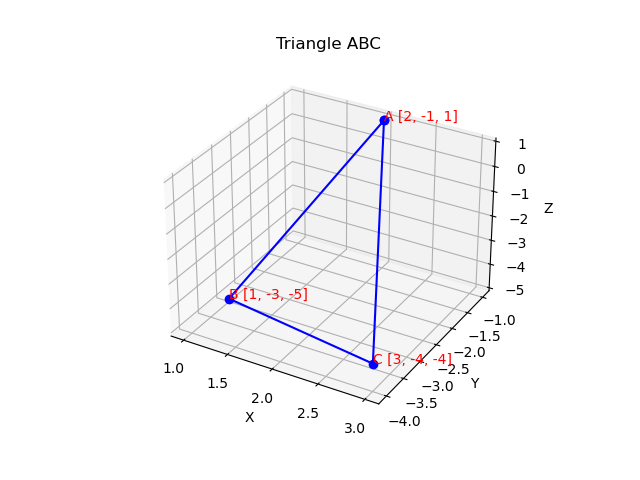
\includegraphics[width = 0.8\columnwidth]{Figs/Figure_1.png}
	\caption{Plot}
    \label{fig:placeholder}
\end{figure}
\end{document}

